%!TEX root = A0.Master.tex
\chapterbegin{Descripción de la aplicación: cliente y servidor}

La aplicación desarrollada en el presente proyecto está compuesta por dos partes fundamentales: el proveedor de datos situado en un servidor remoto, y la aplicación del dispositivo móvil, que pide datos al servidor e interpreta en la pantalla del usuario dichos resultados.

Como ya se ha comentado en el primer capítulo, la parte del servidor no será descrita por completo ya que no entra dentro del ámbito de este Proyecto de Fin de Carrera.

\section{Cliente}
En esta sección nos concentraremos en describir la aplicación cliente que el usuario dispondrá en su iPhone. Este cliente debe proporcionar de manera rápida y eficaz la información que necesita el usuario. Para ello se ha diseñado un sistema de navegación de varios pasos consecutivos, simplificando la UI al máximo para cumplir los requisitos de rapidez y eficacia, teniendo en mente siempre que el usuario utilizará nuestra aplicaciones por un tiempo menor de 30 segundos, ya que se encuentra ocupado comprando en la tienda física. En la figura \ref{fig:esqueleto} se muestra el esqueleto de nuestra aplicación cliente.

\begin{figure}[h]
	\centering
		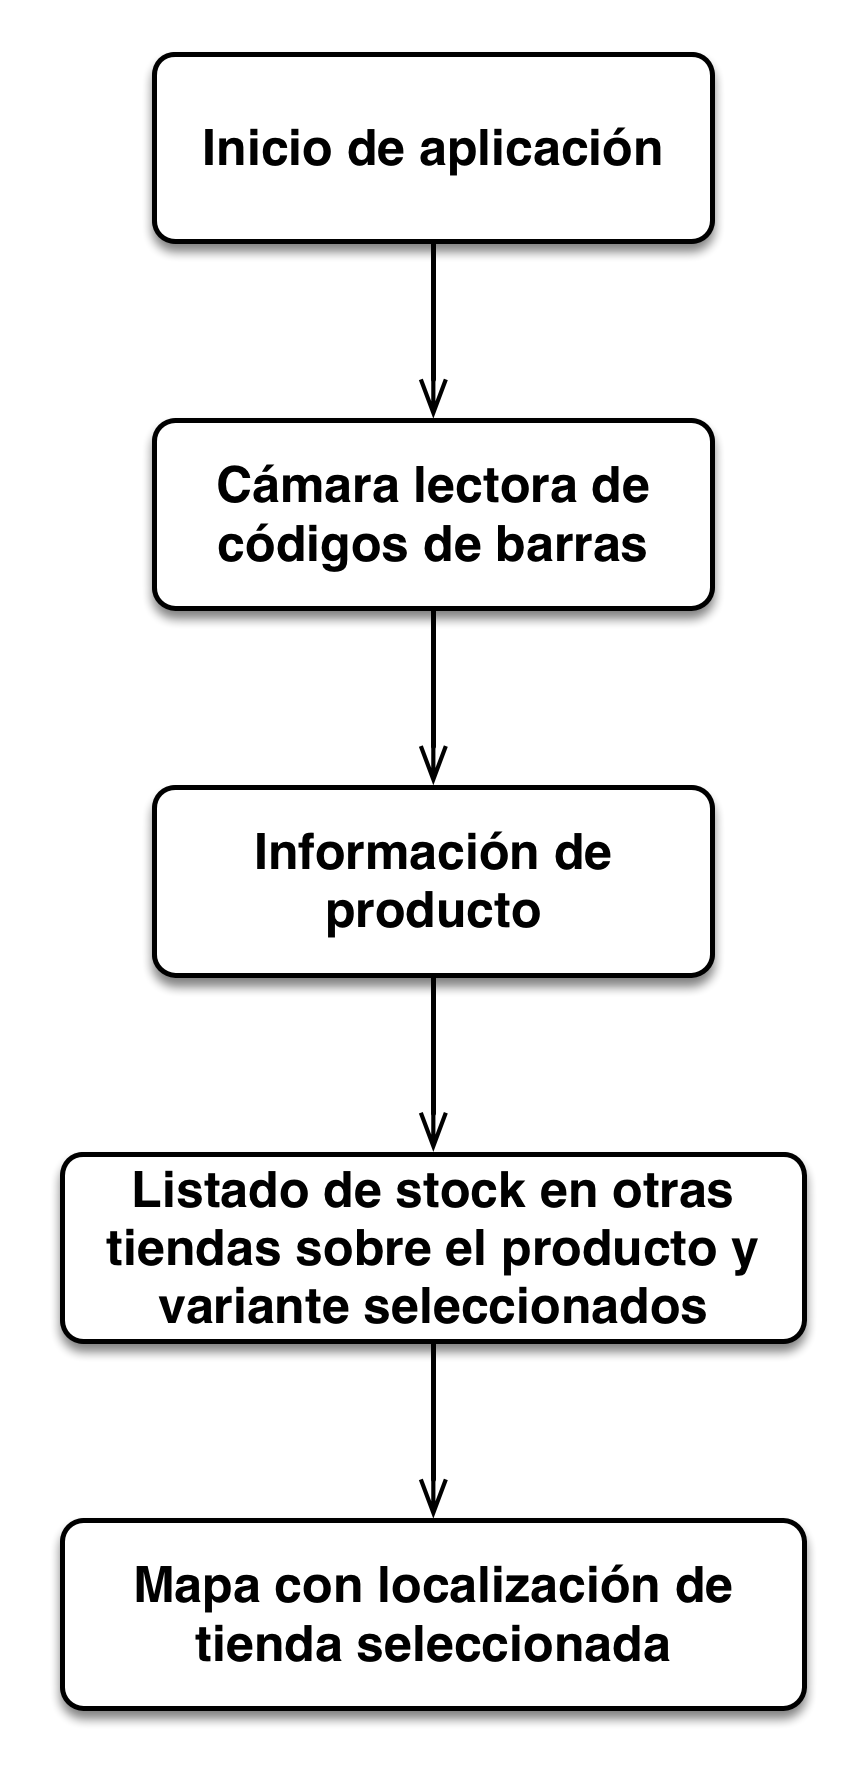
\includegraphics[width=0.3\textwidth]{./img/esqueleto-app.png}
	\caption{Esqueleto de navegación entre pantallas de la aplicación móvil cliente del usuario.}
	\label{fig:esqueleto}
\end{figure}

\subsection{Pantallas del cliente}
La aplicación móvil dispone de una pantalla de inicio, una pantalla que previsualiza la imagen capturada por la cámara trasera del móvil, una pantalla que muestra el producto escaneado, una pantalla que lista las diferentes tiendas con el stock actual de dicho producto, y una mapa que muestra la posición actual del usuario y de la tienda seleccionada en la pantalla anterior.

A continuación se describirá cada una de las pantallas que componen nuestra aplicación. El dispositivo utilizado para el desarrollo es un iPhone 5 con una resolución de 1136x640 píxeles, aunque esto no supone ningún impedimento para mostrar la aplicación en otras resoluciones gracias al uso de AutoLayout.

Esta tecnología permite definir las reglas por las que se rigen los elementos en pantalla (campos de texto, botones, etc.) en vez de definir unas medidas exactas.

\subsubsection{Pantalla de inicio}
La aplicación móvil dispone de una pantalla de inicio que muestra el logotipo de la empresa que ha encargado la creación de la app. Este proceso es requerido por Apple si se desea publicar la aplicación en la App Store. El tiempo que esta pantalla es mostrada dependerá de la velocidad con la que se inicia la aplicación.

%% TO DO: Poner imagen de la UMA y hacer captura.

\subsubsection{Pantalla de inicio: cámara}
Lo primero que verá el usuario en pantalla será la propia imagen de la cámara, lista para capturar un código de barras. El decodificador de barras está programado de manera que únicamente reconozca el formato \emph{Code 128}. En caso de lectura de un código que no pertenezca a ningún producto, se muestra un mensaje de error.

\begin{figure}[h]
	\centering
		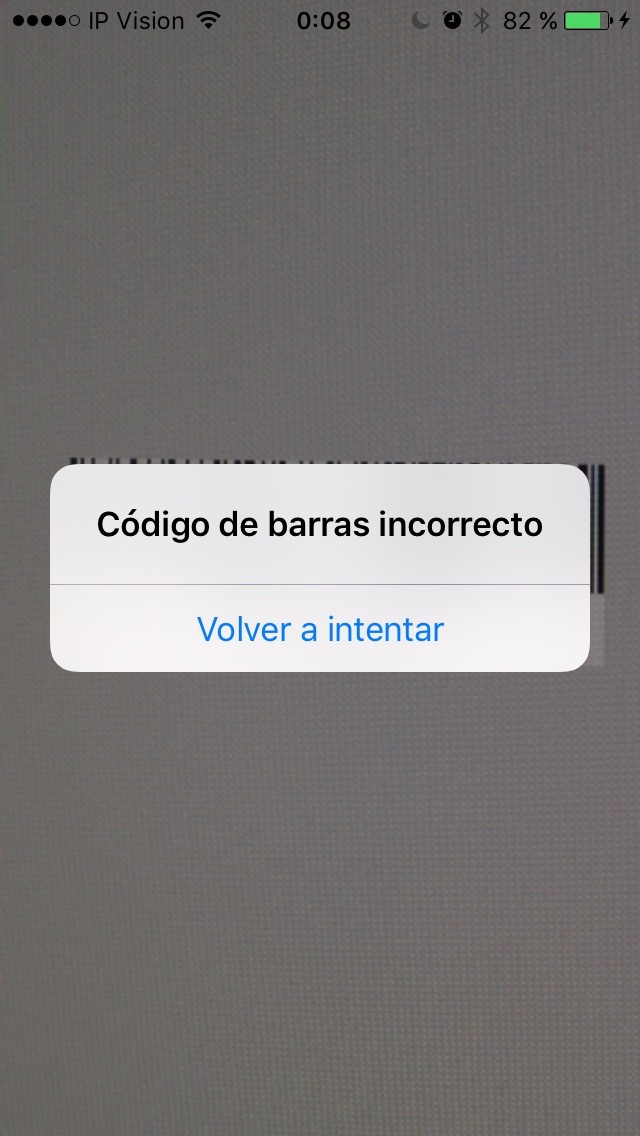
\includegraphics[width=0.4\textwidth]{./img/camara-error.jpg}
	\caption{Mensaje de error mostrado al usuario cuando el código de barras es incorrecto.}
	\label{fig:codigoBarrasError}
\end{figure}

\subsubsection{Pantalla de información de producto}

\subsubsection{Pantalla de lista de tiendas con stock}

\subsubsection{Pantalla de mapa con tienda geolocalizada}

\subsection{Petición y recepción de datos del servidor en el cliente}
Como ya se ha comentado anteriormente, la aplicación cliente realiza peticiones al servidor, que devuelve los datos en formato JSON.

\section{Servidor}

\chapterend